\section{Кластеризация слов из электронных писем}

Кластерный анализ (англ. \textit{Data clustering}) — задача разбиения заданной выборки объектов (ситуаций) на непересекающиеся подмножества, называемые кластерами, так, чтобы каждый кластер состоял из схожих объектов, а объекты разных кластеров существенно отличались.

Кластеризация (обучение без учителя) отличается от классификации (обучения с учителем) тем, что метки исходных объектов изначально не заданы. 

В данной работе мы группируем похожие по смыслу слова с помощью векторного представления слов, полученных с помощью \textit{Word2Vec} \cite{bib5}. 

\textit{Word2Vec} принимает большой текстовый корпус в качестве входных данных и сопоставляет каждому слову вектор, выдавая координаты слов на выходе. Сначала он генерирует словарь корпуса, а затем вычисляет векторное представление слов, «обучаясь» на входных текстах. Векторное представление основывается на контекстной близости: слова, встречающиеся в тексте рядом с одинаковыми словами (а следовательно, имеющие схожий смысл), будут иметь близкие (по косинусному расстоянию) векторы. Полученные векторные представления слов могут быть использованы для обработки естественного языка и машинного обучения.

Текстовый корпус, состоящий из слов из электронных писем, недостаточно большой, чтобы получить хорошие результаты. Поэтому мы использовали предобученный датасет, полученный из постов в \text{Twitter} \cite{bib6}, который был дообучен словами из электронных писем.

Полученные вектора кластеризуются с помощью алгоритма \textit{K-Means}. Он разбивает множество элементов векторного пространства на заранее известное число кластеров $k$. Действие алгоритма таково, что он стремится минимизировать среднеквадратичное отклонение на точках каждого кластера. Основная идея заключается в том, что на каждой итерации перевычисляется центр масс для каждого кластера, полученного на предыдущем шаге, затем векторы разбиваются на кластеры вновь в соответствии с тем, какой из новых центров оказался ближе по выбранной метрике. Алгоритм завершается, когда на какой-то итерации не происходит изменения кластеров.

\newpage


Результаты работы алгоритма. Ближайшие слова к <<\textit{obama}>>:

$ $

\begin{tabular}{ | l | l | }
\hline
Слово & Расстояние \\ \hline
romney & 0.9429854154586792 \\ \hline
barack & 0.9073218107223511 \\ \hline
president & 0.8986026048660278 \\ \hline
clinton & 0.8913119435310364 \\ \hline
hillary & 0.8597259521484375 \\ \hline
say & 0.8407208323478699 \\ \hline
hovv & 0.8315389752388 \\ \hline
\end{tabular}

$ $

Ближайшие слова к <<\textit{trump}>>:

$ $

\begin{tabular}{ | l | l | }
\hline
Слово & Расстояние \\ \hline
appropriator & 0.7439741492271423 \\ \hline
infighter & 0.7368026971817017 \\ \hline
zappos & 0.7316897511482239 \\ \hline
perkins & 0.7260088920593262 \\ \hline
donald & 0.7180437445640564 \\ \hline
buffett &  0.7113708853721619 \\ \hline
bloomberg & 0.7067334651947021 \\ \hline
clinton &  0.7052138447761536 \\ \hline
\end{tabular}

$ $

$  $

Так же была построена интерактивная проекция точек на \textit{2D}-плоскость с помощью алгоритма \textit{t-SNE} \cite{bib7}. \textit{t-SNE} --- это техника нелинейного снижения размерности, хорошо подходящей для вложения данных высокой размерности для визуализации в пространство низкой размерности (двух- или трехмерное). В частности, метод моделирует каждый объект высокой размерности двух- или трёхмерной точкой таким образом, что похожие объекты моделируются близко расположенными точками, а непохожие точки моделируются с большой вероятностью точками, далеко друг от друга отстоящими.

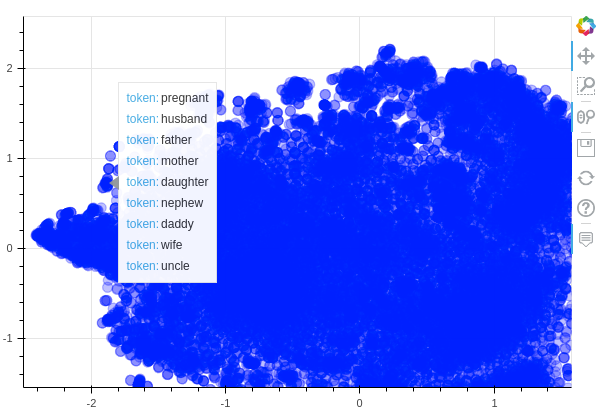
\includegraphics[scale=0.75]{pics/points.png}